\documentclass{book}
\usepackage{etex}
\usepackage{tikz}
\usepackage{ctex,metalogo}\usetikzlibrary{calc}
\setmainfont{Times New Roman}\usepackage{mathdesign}
\usepackage{mtpro2,amsmath,pgfornament,shapepar}
\usepackage[centering,
           top=1.54cm,bottom=0.54cm,right=1.18cm,left=1.18cm,
           headsep=25pt,headheight=20pt]{geometry}
\usetikzlibrary{calc,positioning,intersections}
\setmainfont{Times New Roman}
\usetikzlibrary{arrows}\newsavebox{\bbox}\usetikzlibrary{shapes.geometric,through,decorations.pathmorphing, arrows.meta,quotes,mindmap,shapes.symbols,shapes.arrows,automata,angles,3d,trees,shadows,automata,arrows,
shapes.callouts}
\definecolor{db}{rgb}{0.12,0.53,1}\definecolor{Beige}{rgb}{0.9,0.9,0.9}
\usetikzlibrary{patterns,scopes,math}
\definecolor{mycolor}{RGB}{167,174,245}
\definecolor{redid}{RGB}{248,150,208}
\newcommand{\bd}{\boldsymbol}
\usepackage[hidelinks]{hyperref}
\begin{document}
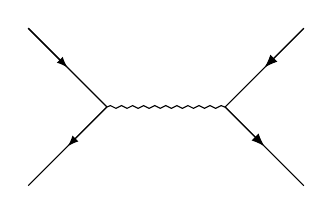
\begin{tikzpicture}[decoration={snake,pre length=0pt,segment length=4pt,amplitude=0.5pt,post length=0pt}]
\draw[-latex](0,1)--(0.5,0.5);\draw(0,1)--(1,0);
\draw[-latex](1,0)--(0.5,-0.5);\draw(1,0)--(0,-1);
\draw[-Latex](3.5,1)--(3,0.5);\draw(3.5,1)--(2.5,0);
\draw[-Latex](2.5,0)--(3,-0.5);\draw(2.5,0)--(3.5,-1);
\draw[decorate](1,0)--(2.5,0);
\end{tikzpicture}
\begin{tikzpicture}[scale=2]
\draw[-Stealth](-1.25,0)--(0,0)node[below left]{$O$}--(1.25,0)node[below]{$x$};
\draw[-Stealth](0,-1.25)--(0,1.25)node[left]{$y$};
\draw(0,0.5)--(1.2,0.5)(0,-0.5)--(-1.2,-0.5);
\filldraw[fill=white](0,0.5)circle(0.5pt)(0,-0.5)circle(0.5pt);
\node[left]at(0,0.5){$1$};\node[right]at(0,-0.5){$-1$};
\fill(0,0)circle(0.5pt);\node at(-0.6,0.6){$y=\operatorname{sgn}x$};
\end{tikzpicture}
\begin{tikzpicture}[scale=0.5]
\draw[-Stealth](-5,0)--(0,0)node[below left]{$O$}--(5.2,0)node[below]{$x$};
\draw[-Stealth](0,-5)--(0,5)node[left]{$y$};
\foreach \x in{-4,-3,...,4}
{\draw(\x,\x)--(\x+1,\x);\draw(\x,0)--(\x,0.05)(0,\x)--(0.05,\x);
\fill(\x,\x)circle(1pt);\draw[white](1,0)--(1,0.05);}
\foreach \x in{-4,-3,...,4}
\filldraw[fill=white](\x+1,\x)circle(1pt);
\foreach \x in{-4,-3,-2,-1,1,2,3,4}
{\node[below]at(\x,0){$\x$};}
\foreach \x in{1,2,3,4}
\node[left]at(0,\x){$\x$};
\foreach \x in{-2,-3,-4}
\node[left]at(0,\x){$\x$};
\node[below left]at(0,-1){$-1$};\node at(-2,2){$y=[x]$};
\end{tikzpicture}
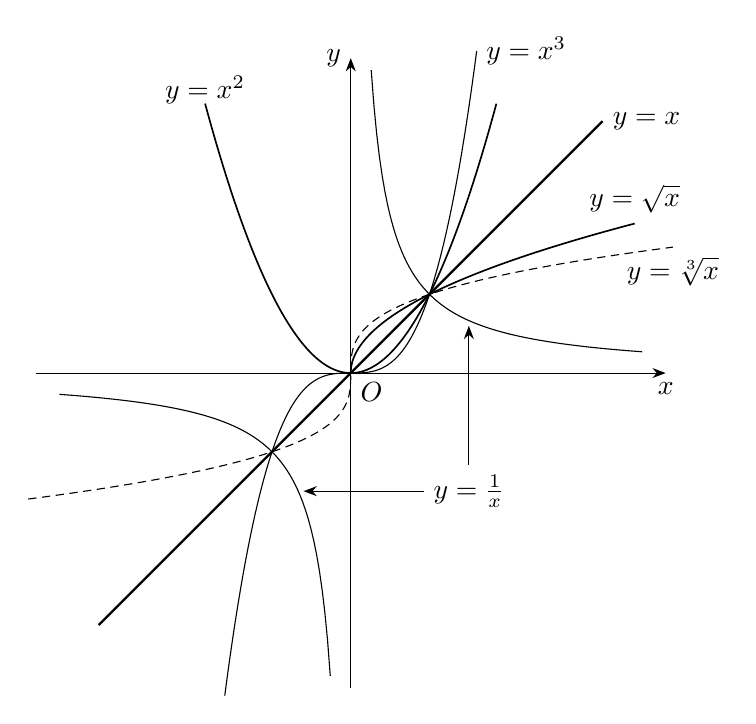
\begin{tikzpicture}[samples=100]
\draw[-Stealth](-4,0)--(0,0)node[below right]{$O$}--(4,0)node[below]{$x$};
\draw[-Stealth](0,-4)--(0,4)node[left]{$y$};
\draw[domain=-1.6:1.6]plot(\x,{(\x)^3})node[right]{$y=x^3$};
\draw[densely dashed,domain=-1.6:1.6]plot({(\x)^3},\x)node[below]{$y=\sqrt[3]x$};
\draw[semithick,domain=0:1.9]plot({(\x)^2},\x)node[above]{$y=\sqrt x$};
\draw[thick,domain=-3.2:3.2]plot(\x,\x)node[right]{$y=x$};
\draw[domain=0.26:3.7]plot(\x,{1/(\x)});
\draw[domain=-0.26:-3.7]plot(\x,{1/(\x)});
\node(a)at(1.5,-1.5){$y=\frac1x$};
\draw[-Stealth](a.west)--(-0.6,-1.5);
\draw[-Stealth](a.north)--(1.5,0.6);
\draw[semithick,domain=-1.85:1.85]plot(\x,{(\x)^2});
\node at(-1.85,3.6){$y=x^2$};
\end{tikzpicture}
\begin{tikzpicture}[samples=100]
\draw[-Stealth](-4,0)--(0,0)node[below left]{$O$}--(4,0)node[below]{$x$};
\draw[-Stealth](0,-4)--(0,4)node[left]{$y$};
\draw[domain=-3.7:1.8]plot(\x,{2^(\x)})node[right]{$y=2^x$};
\draw[domain=3.7:-1.8]plot(\x,{2^(-\x)})node[left]{$y=\left(\frac12\right)^x$};
\node at(-0.3,1){$1$};\node at(1,-0.3){$1$};
\draw[domain=-3.7:1.8]plot({2^(\x)},\x)node[above]{$y=\log_2x$};
\draw[domain=3.7:-1.8]plot({2^(-\x)},\x)node[below]{$y=\log_{\frac12}x$};
\end{tikzpicture}
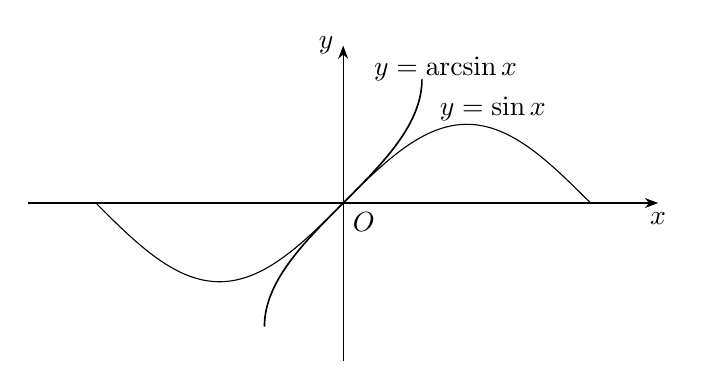
\begin{tikzpicture}[samples=100]
\draw[-Stealth](-4,0)--(0,0)node[below right]{$O$}--(4,0)node[below]{$x$};
\draw[-Stealth](0,-2)--(0,2)node[left]{$y$};
\draw[domain=-pi:pi]plot(\x,{sin(\x r)});
\draw[semithick,domain=-pi/2:pi/2]plot({sin(\x r)},\x);
\node at(1.9,1.2){$y=\sin x$};\node at(1.3,1.7){$y=\arcsin x$};
\end{tikzpicture}
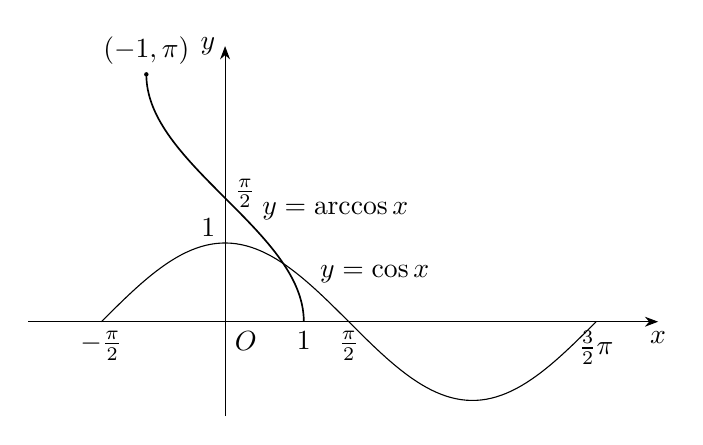
\begin{tikzpicture}[samples=100]
\draw[-Stealth](-2.5,0)--(0,0)node[below right]{$O$}--(5.5,0)node[below]{$x$};
\draw[-Stealth](0,-1.2)--(0,3.5)node[left]{$y$};
\draw[domain=-pi/2:3*pi/2]plot(\x,{cos(\x r)});\node at(1.4,1.4){$y=\arccos x$};
\draw[semithick,domain=0:pi]plot({cos(\x r)},\x);
\node at(1.9,0.6){$y=\cos x$};
\node[left]at(0,1.2){$1$};\
\node[below] at(-pi/2,0){$-\frac\pi2$};
\node[below]at(pi/2,0){$\frac\pi2$};
\node[below]at(1,0){$1$};\node[right]at(0,1.63){$\frac\pi2$};
\node[below]at(3*pi/2,0){$\frac32\pi$};
\fill(-1,pi)circle(0.8pt)node[above]{$(-1,\pi)$};
\end{tikzpicture}

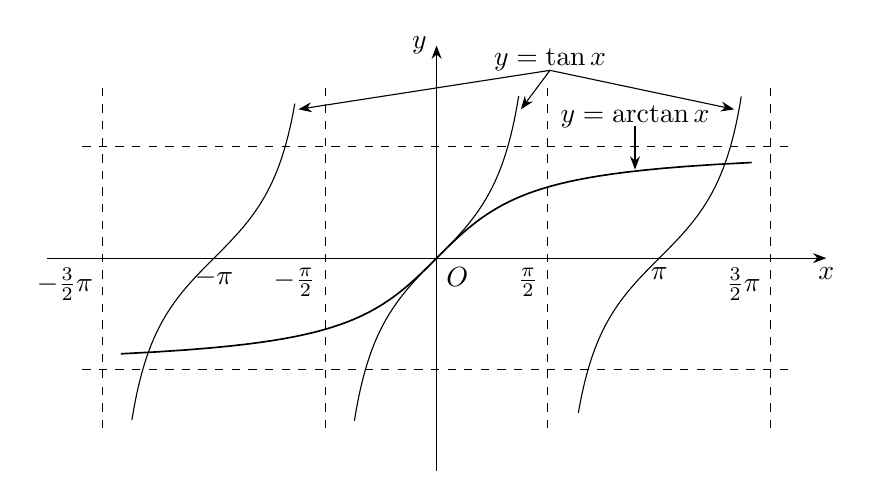
\begin{tikzpicture}[samples=100,scale=0.9]
\draw[-Stealth](-5.5,0)--(0,0)node[below right]{$O$}--(5.5,0)node[below]{$x$};
\draw[-Stealth](0,-3)--(0,3)node[left]{$y$};
\draw[domain=-4.3:-2]plot(\x,{tan(\x r)});
\draw[dashed](-3*pi/2,-2.4)--(-3*pi/2,2.4);
\draw[dashed](-pi/2,-2.4)--(-pi/2,2.4);
\draw[dashed](pi/2,-2.4)--(pi/2,2.4);
\draw[dashed](3*pi/2,-2.4)--(3*pi/2,2.4);
\draw[domain=-1.16:1.16]plot(\x,{tan(\x r)});
\draw[domain=2:4.3]plot(\x,{tan(\x r)});
\node[below left]at(-3*pi/2,0){$-\frac32\pi$};
\node[below left]at(3*pi/2,0){$\frac32\pi$};
\node[below left]at(pi/2,0){$\frac\pi2$};\node[below left]at(-pi/2,0){$-\frac\pi2$};
\node[below]at(pi,0){$\pi$};\node[below]at(-pi,0){$-\pi$};
\node(a)at(1.6,2.8){$y=\tan x$};\node(b) at(2.8,2){$y=\arctan x$};
\draw[semithick,domain=-1.35:1.35]plot({tan(\x r)},\x);
\draw[dashed](-5,pi/2)--(5,pi/2)(-5,-pi/2)--(5,-pi/2);
\draw[-Stealth](2.8,1.87)--(2.8,1.25);
\draw[-Stealth](1.6,2.65)--(-1.95,2.1);
\draw[-Stealth](1.6,2.65)--(1.19,2.1);\draw[-Stealth](1.6,2.65)--(4.2,2.1);
\end{tikzpicture}
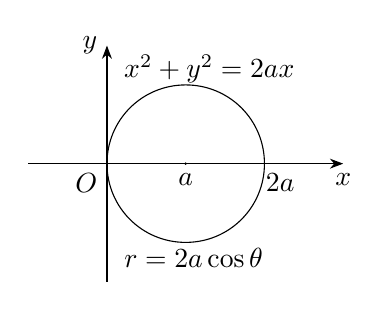
\begin{tikzpicture}[samples=100]
\draw[-Stealth](-1,0)--(0,0)node[below left]{$O$}--(3,0)node[below]{$x$};
\draw[-Stealth](0,-1.5)--(0,1.5)node[left]{$y$};
\draw plot[tension=1,smooth cycle]coordinates{(0,0)(1,1)(2,0)(1,-1)};
\node [below]at(2.2,0){$2a$};\node [below]at(1,0){$a$};
\fill(1,0)circle(0.5pt);
\node at(1.1,-1.2){$r=2a\cos\theta$};
\node at(1.3,1.2){$x^2+y^2=2ax$};
\end{tikzpicture}
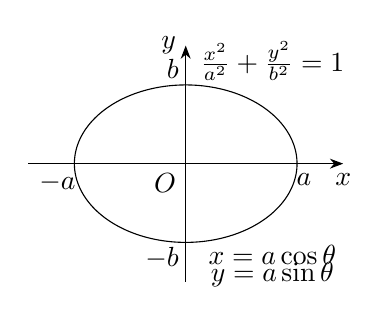
\begin{tikzpicture}[samples=200]
\draw[-Stealth](-2,0)--(0,0)node[below left]{$O$}--(2,0)node[below]{$x$};
\draw[-Stealth](0,-1.5)--(0,1.5)node[left]{$y$};
\draw[domain=0:2*pi]plot({1.414*cos(\x r)},{sin(\x r)});
\node[left=-1pt] at(0,1.2){$b$};\node[left=-1pt] at(0,-1.2){$-b$};
\node[below] at(-1.63,0){$-a$};\node[below] at(1.5,0){$a$};
\node at(1.1,1.3){$\frac{x^2}{a^2}+\frac{y^2}{b^2}=1$};
\node[align=flush center] at(1.1,-1.3){$x=a\cos\theta$\\[-2mm]
$y=a\sin\theta$};
\end{tikzpicture}
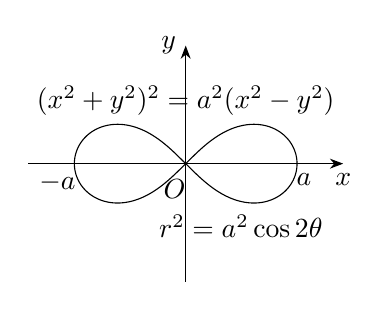
\begin{tikzpicture}[samples=200]
\draw[-Stealth](-2,0)--(2,0)node[below]{$x$};
\draw[-Stealth](0,-1.5)--(0,1.5)node[left]{$y$};
\draw[domain=-pi/4:pi/4]plot({1.414*sqrt(cos(2*\x r))*cos(\x r)},{1.414*sqrt(cos(2*\x r))*sin(\x r)})--(0,0);
\draw[domain=-pi/4:pi/4,rotate=180]plot({1.414*sqrt(cos(2*\x r))*cos(\x r)},{1.414*sqrt(cos(2*\x r))*sin(\x r)})--(0,0);
\node at(-4pt,-9pt){$O$};
\node[below]at(-1.63,0){$-a$};\node[below]at(1.5,0){$a$};
\node at(0,0.8){$(x^2+y^2)^2=a^2(x^2-y^2)$};
\node at(0.7,-0.8){$r^2=a^2\cos2\theta$};
\end{tikzpicture}
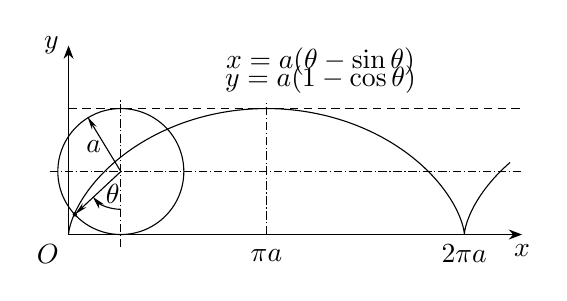
\begin{tikzpicture}[scale=0.8]
\draw[-Stealth](0,0)--(7.2,0)node[below]{$x$};
\draw[-Stealth](0,0)--(0,3)node[left]{$y$};
\node[below left]at(0,0){$O$};
\draw[domain=0:8,samples=200]plot({\x-sin(\x r)},{1-cos(\x r)});
\node[below]at(6.28,0){$2\pi a$};
\draw[densely dashed](0,2)--(7.2,2);
\draw[densely dash dot](-0.3,1)--(7.2,1)(3.1415,0)--(3.1415,2.1)(0.83,-0.2)--(0.83,2.17);
\node[below=2pt]at(3.1415,0){$\pi a$};
\draw (0.83,1)circle(1cm);
\draw[-{Stealth[width=0pt 5]}](0.83,1)--(0.3,1.87);
\node at (0.4,1.4){$a$};
\draw[-{Stealth[width=0pt 5]}](0.83,1)--(0.1,0.32);
\fill(0.1,0.32)circle(1pt);
\draw[-{Stealth[width=0pt 6]}](0.83,0.4)arc(-90:-138:0.6);
\node at(0.7,0.64){$\theta$};
\node[align=center] at(4,2.6){$x=a(\theta-\sin\theta)$\\[-2mm]
$y=a(1-\cos\theta)$};
\end{tikzpicture}

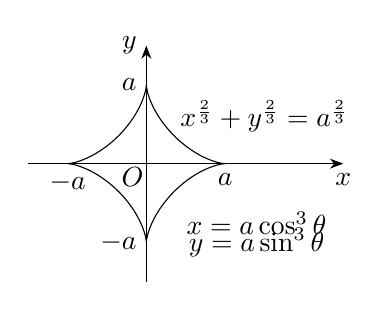
\begin{tikzpicture}[samples=200]
\draw[-Stealth](-1.5,0)--(2.5,0)node[below]{$x$};
\draw[-Stealth](0,-1.5)--(0,1.5)node[left]{$y$};
\draw[domain=0:2*pi]plot({(cos(\x r))^3},{(sin(\x r))^3});
\node[left]at(0,1){$a$};\node[left]at(0,-1){$-a$};
\node[below]at(1,0){$a$};\node[below]at(-1,0){$-a$};
\node at(1.5,0.6){$x^{\frac23}+y^{\frac23}=a^{\frac23}$};
\node[align=center]at(1.4,-0.9){$x=a\cos^3\theta$\\[-2mm]$y=a\sin^3\theta$};
\node at(-5pt,-5pt){$O$};
\end{tikzpicture}
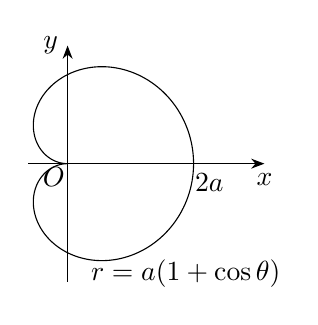
\begin{tikzpicture}[samples=200]
\draw[-Stealth](-0.5,0)--(2.5,0)node[below]{$x$};
\draw[-Stealth](0,-1.5)--(0,1.5)node[left]{$y$};
\draw[domain=-pi:pi]plot({1.6*cos(\x/2 r)*cos(\x r)},{1.6*cos(\x/2 r)*sin(\x r)});
\node at(-5pt,-5pt){$O$};\node[below]at(1.8,0){$2a$};
\node at(1.5,-1.4){$r=a(1+\cos\theta)$};
\end{tikzpicture}
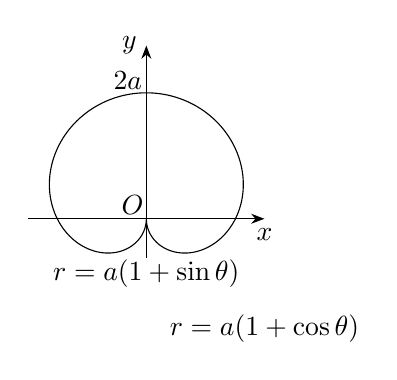
\begin{tikzpicture}[samples=200]
\draw[-Stealth](-1.5,0)--(1.5,0)node[below]{$x$};
\draw[-Stealth](0,-0.5)--(0,2.2)node[left]{$y$};
\draw[domain=-pi:pi,rotate=90]plot({1.6*cos(\x/2 r)*cos(\x r)},{1.6*cos(\x/2 r)*sin(\x r)});
\node at(-5pt,5pt){$O$};\node[left=-2pt]at(0,1.75){$2a$};
\node at(1.5,-1.4){$r=a(1+\cos\theta)$};
\node at(0,-0.7){$r=a(1+\sin\theta)$};
\end{tikzpicture}
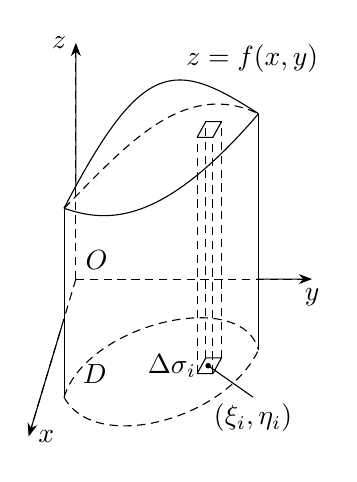
\begin{tikzpicture}[x={(-0.3cm,-1cm)},y={(1cm,0cm)},z={(0cm,1cm)}]
\draw[densely dashed,-Stealth](0,0,0)node[above right]{$O$}--(0,3,0)node[below]{$y$};
\draw[densely dashed,-Stealth](0,0,0)--(0,0,3)node[left]{$z$};
\draw[densely dashed,-Stealth](0,0,0)--(2,0,0)node[right]{$x$};
\begin{scope}[canvas is xy plane at z=0]
\draw[densely dashed,bend left=75](1.5,0.3)to(0.9,2.59);
\draw[densely dashed,bend right=65](1.5,0.3)to(0.9,2.59);
\end{scope}
\draw(1.5,0.3,0)--(1.5,0.3,2.4)(0.9,2.59,0)--(0.9,2.59,3);
\draw(1.5,0.3,2.4)..controls(1.2,1.2,4)and(1.2,1.6,4)..(0.9,2.59,3);
\draw[densely dashed,out=45,in=155](1.5,0.3,2.4)to(0.9,2.59,3);
\draw[smooth](0.9,2.59,3)
..controls(1.6,1.6,2.3)and(1.6,0.9,2.3)..(1.5,0.3,2.4);
\node at(1.2,0.6,0){$D$};\node at(1.1,1.55,0){$\Delta\sigma_i$};
\draw(1.2,1.9,0)--(1.2,2.1,0)--(1,2.15,0)--(1,1.95,0)--(1.2,1.9,0);
\draw(1.2,1.9,3)--(1.2,2.1,3)--(1,2.15,3)--(1,1.95,3)--(1.2,1.9,3);
\draw[densely dashed](1.2,1.9,0)--(1.2,1.9,3)(1.2,2.1,0)--(1.2,2.1,3)(1,2.15,0)--(1,2.15,3)
(1,1.95,0)--(1,1.95,3);
\fill(1.1,2.01,0)circle(1pt){};\draw(1.1,2.01,0)--(1.5,2.7,0)node[below=-1pt]{$(\xi_i,\eta_i)$};
\draw(0,0,1.18)--(0,0,2.9)(0,2.3,0)--(0,2.9,0)(0.6,0,0)--(1.9,0,0);
\node at(0.2,2.3,3){$z=f(x,y)$};
\end{tikzpicture}
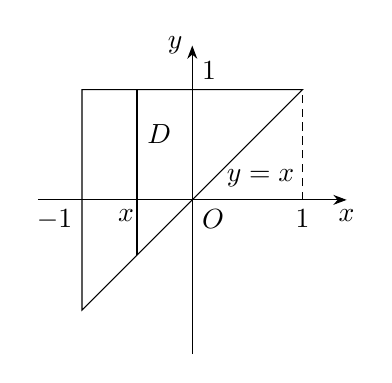
\begin{tikzpicture}[>=Stealth,scale=1.4]
\draw[->](-1.4,0)--(0,0)node[below right]{$O$}--(1.4,0)node[below]{$x$};
\draw[->](0,-1.4)--(0,1.4)node[left]{$y$};
\draw(1,1)--(-1,1)--(-1,-1)--cycle;
\node[below left]at(-1,0){$-1$};\node[below]at(1,0){$1$};
\node[above right]at(0,1){$1$};
\draw[densely dashed](1,0)--(1,1);
\draw[semithick](-0.5,1)--(-0.5,-0.5);\node at(0.62,0.2){$y=x$};
\node at(-0.3,0.6){$D$};\node[below] at(-0.6,0){$x$};
\end{tikzpicture}
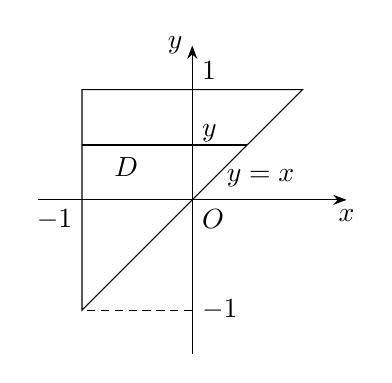
\begin{tikzpicture}[>=Stealth,scale=1.4]
\draw[->](-1.4,0)--(0,0)node[below right]{$O$}--(1.4,0)node[below]{$x$};
\draw[->](0,-1.4)--(0,1.4)node[left]{$y$};
\draw(1,1)--(-1,1)--(-1,-1)--cycle;
\node[below left]at(-1,0){$-1$};;
\node[above right]at(0,1){$1$};
\draw[densely dashed](0,-1)node[right]{$-1$}--(-1,-1);
\node at(0.62,0.2){$y=x$};
\node at(-0.6,0.3){$D$};\draw[semithick](-1,0.5)--(0.5,0.5);
\node[right]at(0,0.6){$y$};
\end{tikzpicture}
\begin{tikzpicture}[>=Stealth,scale=1.3]
\draw[->](0,0)node[below]{$O$}--(3,0)node[below]{$x$};
\draw[->](0,0)--(0,3)node[left]{$y$};
\draw(1,1)--(2,2)--(2,1)--cycle;
\draw[densely dashed](1,1)--(1,0)node[below]{$1$}(2,1)--(2,0)node[below]{$2$}
(1.4,1)node[below right=-1pt and -2pt]{$y{=}1$}--(1.4,0)node[below=2pt]{$x$};
\draw(1.4,1)--(1.4,1.4)node[above left=-4pt and -4pt]{$y{=}x$};
\node at(1.7,1.3){$D$};
\end{tikzpicture}
\begin{tikzpicture}[>=Stealth,scale=1.3]
\draw[->](0,0)node[below]{$O$}--(3,0)node[below]{$x$};
\draw[->](0,0)--(0,3)node[left]{$y$};
\draw(1,1)--(2,2)--(2,1)--cycle;
\draw[densely dashed](1,1)--(0,1)node[left]{$1$}(2,2)--(0,2)node[left]{$2$};
\draw[densely dashed](1.6,1.6)--(0,1.6)node[left]{$y$};
\node at(1.4,1.8){$x{=}y$};\node at(2.3,1.85){$x{=}2$};
\node at(1.7,1.3){$D$};\draw(1.6,1.6)--(2,1.6);
\end{tikzpicture}
\begin{tikzpicture}[>=Stealth,scale=1.3]
\draw[->](0,0)node[below]{$O$}--(3,0)node[below]{$x$};
\draw[->](0,0)--(0,3)node[left]{$y$};
\draw(1.7,0)node[below]{$R$}arc(0:90:1.7);
\node at(0.5,0.6){$D$};\draw(1,1.37)--(1,0)node[below]{$x$};
\node at(2.05,1.37){$y{=}\sqrt{R^2-x^2}$};
\end{tikzpicture}
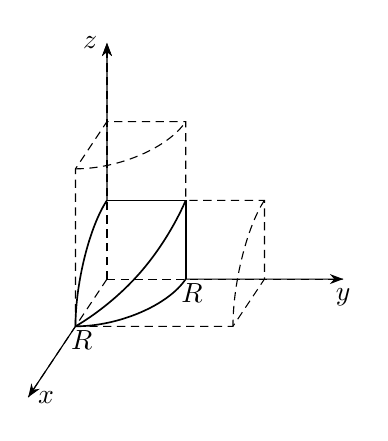
\begin{tikzpicture}[>=Stealth,x={(-0.4cm,-0.6cm)},y={(1cm,0cm)},z={(0cm,1cm)}]
\draw[->,densely dashed](0,0,0)--(0,3,0)node[below]{$y$};
\draw[->,densely dashed](0,0,0)--(0,0,3)node[left]{$z$};
\draw[->,densely dashed](0,0,0)--(2.5,0,0)node[right]{$x$};
\draw[semithick](0,1,0)--(0,1,1)--(0,0,1);
\node at(1.3,0.2,0){$R$};\node at(0.3,1.2,0){$R$};
\draw[densely dashed](1,0,0)--(1,2,0)--(0,2,0)--(0,2,1)--(0,1,1);
\begin{scope}[canvas is xy plane at z=0]
\draw[semithick](1,0)arc(0:90:1);
\end{scope}
\begin{scope}[canvas is zx plane at y=0]
\draw[semithick](1,0)arc(0:90:1);
\end{scope}
\begin{scope}[canvas is zx plane at y=2]
\draw[densely dashed](1,0)arc(0:90:1);
\end{scope}
\begin{scope}[canvas is xy plane at z=2]
\draw[densely dashed](1,0)arc(0:90:1);
\end{scope}
\draw[densely dashed](1,0,0)--(1,0,2)--(0,0,2)--(0,1,2)--(0,1,0);
\draw[->](1,0,0)--(2.5,0,0)(0,1,0)--(0,3,0)(0,0,1)--(0,0,3);
\draw[semithick] plot[smooth,tension=1]coordinates{(1,0,0)(0.7,0.7,0.5)(0,1,1)};
\end{tikzpicture}
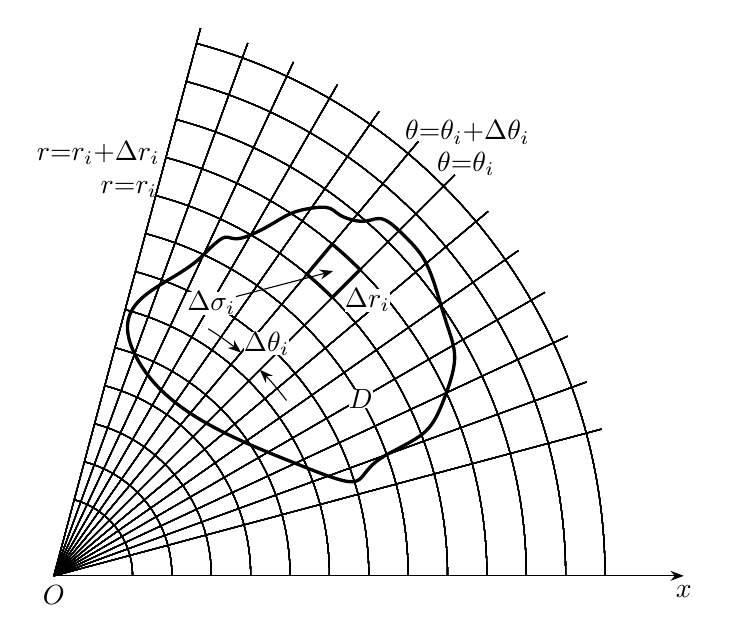
\begin{tikzpicture}[>=Stealth]
\draw[->](0,0)node[below]{$O$}--(8,0)node[below]{$x$};
\foreach \x in{15,20,...,75}
\foreach \y in{1,1.5,...,7}
{\draw(0,0)--({7.2*cos(\x)},{7.2*sin(\x)});\draw(\y,0)arc(0:75:\y);}
\draw[very thick]plot[smooth cycle,tension=1]coordinates{(23:3.5)(20:4.5)(25:5.5)
(35:6)(45:6.2)(50:5.9)(55:5.7)(60:5)(65:4.5)(70:3)};
\draw[very thick](45:5)--(45:5.5)arc(45:50:5.5)--(50:5)arc(50:45:5);
\node(a)[fill=white,inner sep=0pt]at(60:4){$\Delta\sigma_i$};
\draw[->](a)--(47.5:5.25);\node[fill=white,inner sep=0pt] at(41.3:5.3){$\Delta r_i$};
\node[fill=white,inner sep=0pt]at(30:4.5){$D$};
\node[fill=white,inner sep=0pt]at(47.5:4){$\Delta\theta_i$};
\draw[->](37:3.7)arc(37:45:3.7);
\draw[->](58:3.7)arc(58:50:3.7);
\node at(45:7.4){$\theta{=}\theta_i$};
\node at(47:7.7){$\theta{=}\theta_i{+}\Delta\theta_i$};
\node at(79:5){$r{=}r_i$};\node at(84:5.4){$r{=}r_i{+}\Delta r_i$};
\end{tikzpicture}
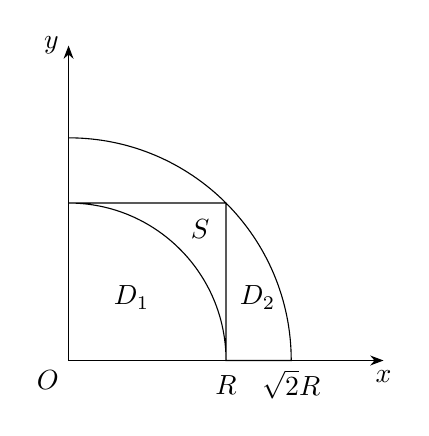
\begin{tikzpicture}
\draw[-Stealth](0,0)node[below left]{$O$}--(4,0)node[below]{$x$};
\draw[-Stealth](0,0)--(0,4)node[left]{$y$};
\draw(2,0)arc(0:90:2)--(2,2)--(2,0)node[below=2pt]{$R$}
--(2.828,0)node[below]{$\sqrt2R$}arc(0:90:2.828);
\node at(0.8,0.8){$D_1$};\node at(1.67,1.67){$S$};
\node at(2.4,0.8){$D_2$};
\end{tikzpicture}
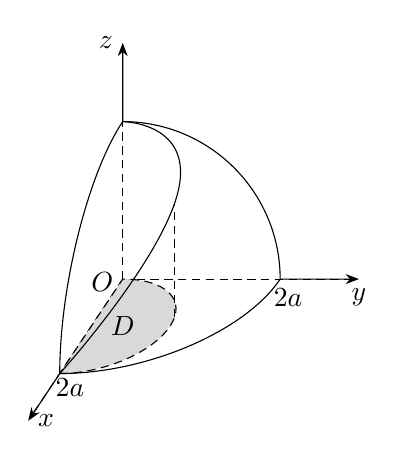
\begin{tikzpicture}[>=Stealth,x={(-0.4cm,-0.6cm)},y={(1cm,0cm)},z={(0cm,1cm)}]
\draw[densely dashed,->](0,0,0)--(3,0,0)node[right]{$x$};
\draw[densely dashed,->](0,0,0)--(0,3,0)node[below]{$y$};
\draw[densely dashed,->](0,0,0)--(0,0,3)node[left]{$z$};
\begin{scope}[canvas is xy plane at z=0]
\filldraw[densely dashed,fill=gray!30](2,0)arc(0:180:1)--cycle;
\draw(2,0)arc(0:90:2);
\node at(2.3,0.25){$2a$};
\end{scope}
\begin{scope}[canvas is zx plane at y=0]
\draw(2,0)arc(0:90:2);
\end{scope}
\begin{scope}[canvas is yz plane at x=0]
\draw(2,0)arc(0:90:2);
\end{scope}
\draw[densely dashed](0.8,0.9798,0)--(0.8,0.9798,1.45);
\draw plot[smooth,tension=1]coordinates{(2,0,0)(1,1.1,1.7)(0,0,2)};
\node at(0.4,-0.1,0.2){$O$};
\draw(0,0,2)--(0,0,2.9)(0,2,0)--(0,2.9,0)(2,0,0)--(2.9,0,0);
\node at(1,0.4,0){$D$};
\node[below]at(0,2.1,0){$2a$};
\end{tikzpicture}
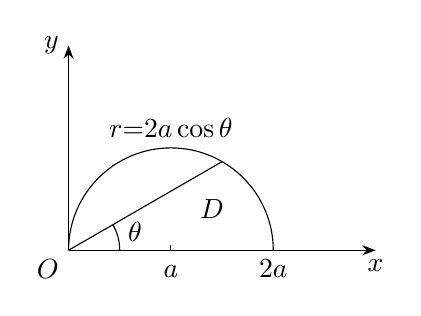
\begin{tikzpicture}[>=Stealth,scale=1.3]
\draw[->](0,0)node[below left]{$O$}--(3,0)node[below]{$x$};
\draw[->](0,0)--(0,2)node[left]{$y$};
\draw(2,0)node[below]{$2a$}arc(0:180:1);
\draw(1,0.05)--(1,0)node[below=2pt]{$a$};
\draw(0,0)--(1.5,0.866);\draw(0.5,0)arc(0:30:0.5);
\node at(1.4,0.4){$D$};\node at(0.65,0.18){$\theta$};
\node at(1,1.2){$r{=}2a\cos\theta$};
\end{tikzpicture}
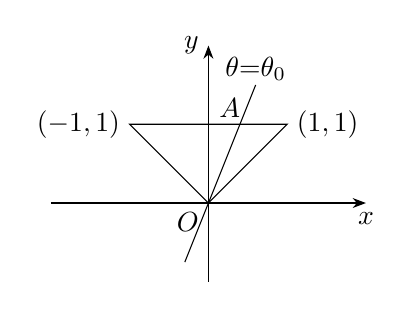
\begin{tikzpicture}
\draw[-Stealth](-2,0)--(0,0)node[below left]{$O$}--(2,0)node[below]{$x$};
\draw[-Stealth](0,-1)--(0,2)node[left]{$y$};
\draw(-1,1)node[left]{$(-1,1)$}--(1,1)node[right]{$(1,1)$}--(0,0)--cycle;
\draw[domain=-0.3:0.6]plot(\x,{2.5*(\x)})node[above=-2pt]{$\theta{=}\theta_0$};
\node at(0.27,1.2){$A$};
\end{tikzpicture}
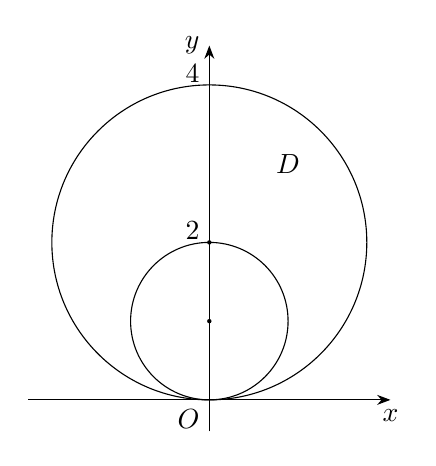
\begin{tikzpicture}[>=Stealth,samples=100]
\draw[->](-2.3,0)--(2.3,0)node[below]{$x$};
\draw[->](0,-0.4)--(0,0)node[below left]{$O$}--(0,4.5)node[left]{$y$};
\draw(0,1)circle(1);\draw(0,2)circle(2);
\fill(0,1)circle(0.8pt);\fill(0,2)circle(0.8pt);
\node[left]at(0,2.15){$2$};\node[left]at(0,4.15){$4$};
\node at(1,3){$D$};
\end{tikzpicture}
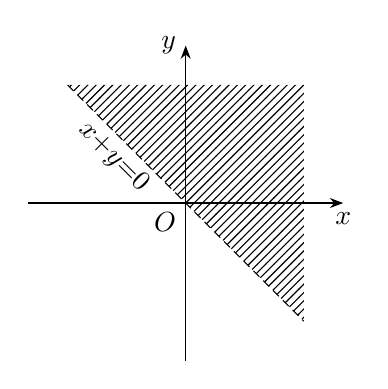
\begin{tikzpicture}[>=Stealth,samples=100]
\draw[->](-2,0)--(0,0)node[below left]{$O$}--(2,0)node[below]{$x$};
\draw[->](0,-2)--(0,2)node[left]{$y$};
\fill[pattern=north east lines](-1.5,1.5)--(1.5,1.5)--(1.5,-1.5)--cycle;
\draw[densely dashed](-1.5,1.5)--node[below=-1pt,sloped,near start]{$x{+}y{=}0$}(1.5,-1.5);
\end{tikzpicture}
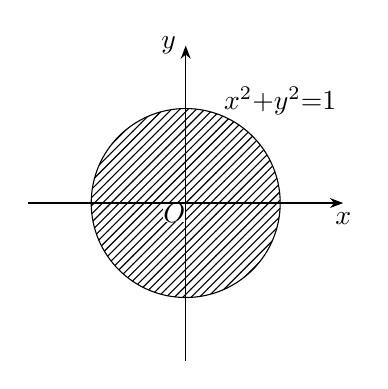
\begin{tikzpicture}[>=Stealth]
\draw[->](0,-2)--(0,2)node[left]{$y$};
\filldraw[pattern=north east lines](0,0)circle(1.2);
\draw[->](-2,0)--(0,0)node[below left,fill=white,inner sep=0pt]{$O$}--(2,0)node[below]{$x$};
\node at(1.2,1.3){$x^2{+}y^2{=}1$};
\end{tikzpicture}

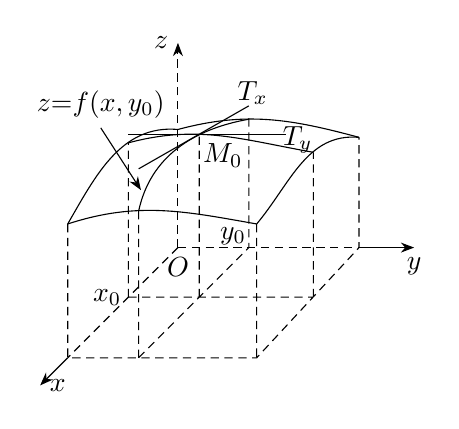
\begin{tikzpicture}[>=Stealth,x={(-0.7cm,-0.7cm)},y={(1cm,0cm)},z={(0cm,1cm)}]
\draw[->](0,0,0)node[below]{$O$}[densely dashed]--(0,0,2.6)node[left]{$z$};
\draw(0,0,0)[densely dashed]--(0,2.35,0);
\draw[->](0,2.35,0)--(0,3,0)node[below]{$y$};
\draw(0,0,0)[densely dashed]--(2,0,0);
\draw[->](2,0,0)--(2.5,0,0)node[right]{$x$};
\draw[densely dashed](2,0,1.7)--(2,0,0)--(2,2.4,0)--(0,2.3,0)--(0,2.3,1.4)
(0.9,0,0)--(0.9,2.35,0)(0,0.9,1.64)--(0,0.9,0)--(2,0.9,0)
(0.9,0,0)node[left=-1pt]{$x_0$}--(0.9,0,1.96)(0.9,2.35,0)--(0.9,2.35,1.84)
(2,0.9,0)--(2,0.9,1.9)(0.9,0.9,0)--(0.9,0.9,2.1)
(2,2.4,1.7)--(2,2.4,0);
\node at(0,0.7,0.15){$y_0$};
\draw[out=18,in=170](2,0,1.7)to(2,2.4,1.7);
\draw[out=60,in=175](2,0,1.7)to(0,0,1.5);
\draw[out=15,in=165](0,0,1.5)to(0,2.3,1.4);
\draw[out=50,in=175](2,2.4,1.7)to(0,2.3,1.4);
\draw[out=15,in=170](0.9,0,1.96)to(0.9,2.35,1.84);
\draw[out=78,in=-170](2,0.9,1.86)to(0,0.9,1.63);
\begin{scope}[canvas is xz plane at y=0.9]
\draw[samples=100,domain=0:2]plot(\x,{2.07+0.3*(\x-0.9)});
\end{scope}
\node at(0,0.95,1.96){$T_x$};
\begin{scope}[canvas is yz plane at x=0.9]
\draw[samples=100,domain=0:2]plot(\x,2.07);
\node at(1.2,1.8){$M_0$};
\end{scope}
\node at(0.9,2.15,2){$T_y$};
\node (a)at(1.4,0,2.8){$z{=}f(x,y_0)$};
\draw[->](a.south)--(2.1,1,2.2);
\end{tikzpicture}
\begin{tikzpicture}
\tikzfading[name =fade inside,inner color=black!100,outer color=black!40]
\fill[black!20](0,0)rectangle(4,4);
\pattern[pattern=checkerboard,pattern color=black!30](0,0)rectangle(4,4);
\shade[ball color=red](3,3)circle(0.8);
\shade[ball color=white,path fading=fade inside](2,2)circle(1.8);
\node[fill=cyan,path fading=east]at(2,2){\heiti 透明度};
\end{tikzpicture}
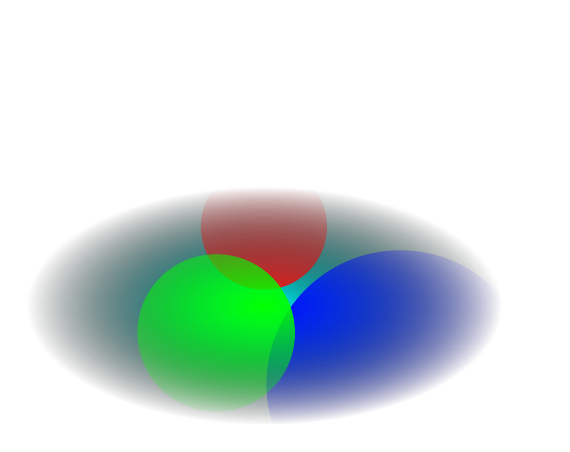
\begin{tikzpicture}
\tikzfading[name =fade out,inner color=black!0,outer color=black!100]
\path[use as bounding box](-3,-1.5)rectangle(3,1.5);
\filldraw[scope fading=fade out,inner color=cyan,outer color=black]
(-3,-1.5)rectangle(3,1.5);
\fill[red](90:1)circle(0.8);\fill[blue](-30:2)circle(1.7);
\fill[green](210:0.7)circle(1);
\end{tikzpicture}
\tikz\node[fill=cyan,scope fading=south,fading angle=45,text width=3cm]
{
This is some text taht will fade out as as we go right and down. It is pretty hard to
achieve this effect in other ways.
};
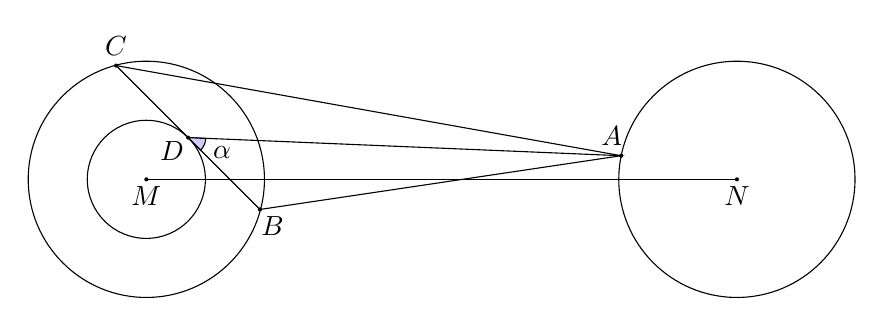
\begin{tikzpicture}[scale=1.5]
\coordinate(a)at(0,0);\coordinate(b)at(5,0);
\draw(0,0)node[below=-1pt]{$M$}circle(1);\draw(0,0)circle(0.5);
\draw(5,0)node[below=-1pt]{$N$}circle(1);
\draw(a)--(b);\node[below left=-2pt and -2pt]at(45:0.5){$D$};
\coordinate(c)at(45:0.5);\coordinate(d)at(4.02,0.2);
\draw[domain=-0.256:0.962]plot(\x,0.707-\x);
\draw(c)--(d);
\coordinate(e)at(-0.256,0.963);\coordinate(f)at(0.962,-0.255);
\draw(e)node[above]{$C$}--(d)--(f)node[below right=-1pt and -3pt]{$B$};
\node[above]at(3.94,0.2){$A$};
\foreach \x in{a,b,c,d,e,f}
\fill(\x)circle(0.5pt);
\filldraw[fill=blue!20]($(c)+(-45:0.15)$)arc(-45:-3:0.15)--(c)--cycle;
\node at(0.64,0.23){$\alpha$};
\end{tikzpicture}
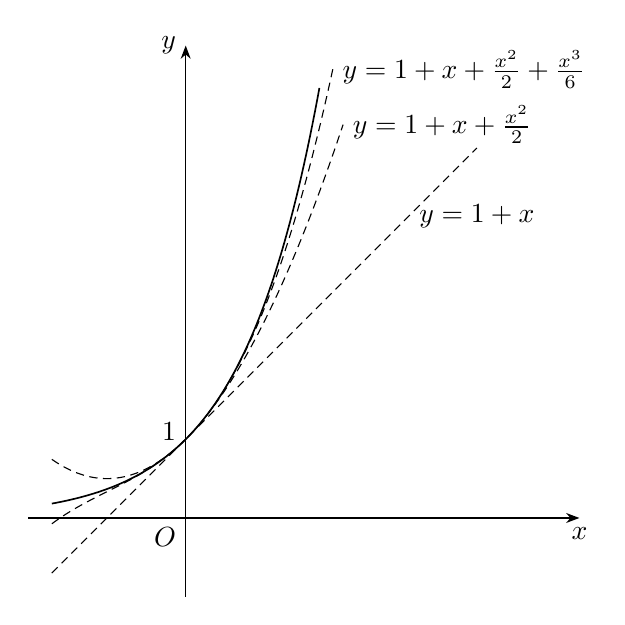
\begin{tikzpicture}[>=Stealth,samples=200]
 \draw[->](-2,0)--(5,0)node[below]{$x$};\draw[->](0,-1)--(0,6)node[left]{$y$};
 \node[below left]{$O$};\node[left]at(0,1.1){$1$};
 \draw[domain=-1.7:1.7,semithick]plot(\x,{e^(\x)});
 \begin{scope}[densely dashed]
 \draw[domain=-1.7:3.7]plot(\x,\x+1)node[below=0.6cm]{$y=1+x$};
 \draw[domain=-1.7:2]plot(\x,{1+\x+(\x)^2/2})node[right]{$y=1+x+\frac{x^2}2$};
  \draw[domain=-1.7:1.87]plot(\x,{1+\x+(\x)^2/2+(\x)^3/6})node[right]
  {$y=1+x+\frac{x^2}2+\frac{x^3}6$};
 \end{scope}
\end{tikzpicture}

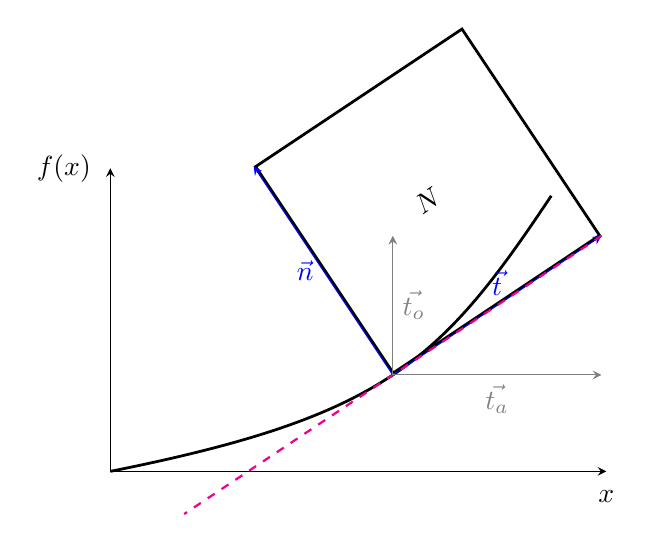
\begin{tikzpicture}[allow upside down,scale=0.7]
\draw [<->,>=stealth] (0,5.5) node [label = left:{$f(x)$}]{} -- (0,0) -- (9,0) node[label = below:{$x$}]{};

 % 将路径画出来,然后选择切点位置为 0.5
\draw[black,line width=1pt] (0,0) .. controls (5,1) and  (6,2) .. (8,5)
      node[sloped,inner sep=0cm,above,pos=0.5,
      anchor=south west,draw,
      minimum size=3.15cm](N){$N$};
 % 绕 N 建立局部的参照点
\path (N.south west)%
           edge[-stealth,blue] node[left] {$\vec{ n}$} (N.north west)
           edge[-stealth,blue] node[above] {$\vec{ t}$} (N.south east);
\path [draw,magenta,thick,dashed](N.south east)--(N.south west) -- ($(N.south west)!1!180:(N.south east)$);

 % 灰色线为点 N 所在垂直的直角坐标系
\draw[-stealth,gray]  (N.south west)  --%
      node[below] {$\vec{t_a}$} (N.south west -| N.south east);
\draw[-stealth,gray]  (N.south west)  --%
      node[right] {$\vec{t_o}$} (N.south west |- N.south east);

\end{tikzpicture}

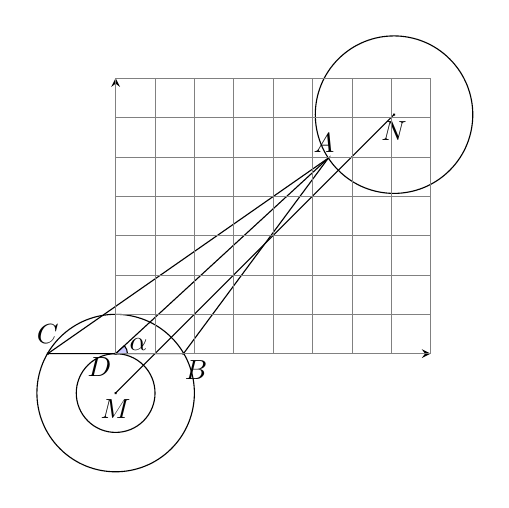
\begin{tikzpicture}
\begin{scope}[rotate=45]
\coordinate(a)at(0,0);\coordinate(b)at(5,0);
\draw(0,0)node[below=-1pt]{$M$}circle(1);\draw(0,0)circle(0.5);
\draw(5,0)node[below=-1pt]{$N$}circle(1);
\draw(a)--(b);\node[below left=-2pt and -2pt]at(45:0.5){$D$};
\coordinate(c)at(45:0.5);\coordinate(d)at(4.02,0.2);
\draw[domain=-0.256:0.962]plot(\x,0.707-\x);
\draw(c)--(d);
\coordinate(e)at(-0.256,0.963);\coordinate(f)at(0.962,-0.255);
\draw(e)node[above]{$C$}--(d)--(f)node[below right=-1pt and -3pt]{$B$};
\node[above]at(3.94,0.2){$A$};
\foreach \x in{a,b,c,d,e,f}
\fill(\x)circle(0.5pt);
\filldraw[fill=blue!20]($(c)+(-45:0.15)$)arc(-45:-3:0.15)--(c)--cycle;
\node at(0.64,0.23){$\alpha$};
\end{scope}
\draw[-stealth](0,0.5)--(4,0.5);
\draw[-stealth](0,0.5)--(0,4);
\draw[help lines,step=0.5cm](0,0.5)grid(4,4);
\end{tikzpicture}
\begin{tikzpicture}[>=Stealth]
\draw[->](0,0)node[below=-1pt]{$O$}--(2.5,0)node[below]{$y$};
\draw[->](0,0)--(0,2.5)node[left]{$z$};
\draw[->](0,0)--(-1.5,-1)node[below=-1pt]{$x$};
\draw[bend left=40,semithick](-0.8,1.5)node[above=-1pt]{$\Gamma$}to(2,1.7);
\node at(0.9,2.3){$M$};
\draw[-Stealth](0,0)--node[right]{$\boldsymbol r$}(0.85,2.13);
\end{tikzpicture}
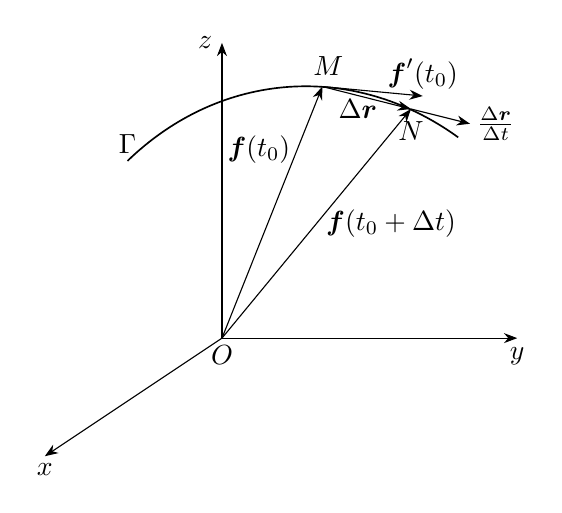
\begin{tikzpicture}[>=Stealth,scale=1.5]
\draw[->](0,0)node[below=-1pt]{$O$}--(2.5,0)node[below]{$y$};
\draw[->](0,0)--(0,2.5)node[left]{$z$};
\draw[->](0,0)--(-1.5,-1)node[below=-1pt]{$x$};
\draw[bend left=40,semithick](-0.8,1.5)node[above=-1pt]{$\Gamma$}to(2,1.7);
\node at(0.9,2.3){$M$};
\draw[->](0,0)--node[left=-1pt,near end]{$\bd f(t_0)$}(0.85,2.13);
\draw[->](0.85,2.13)--(1.7,2.05)node[above=-1pt]{$\bd f'(t_0)$};
\draw[->](0,0)--node[right]{$\bd f(t_0+\Delta t)$}(1.6,1.94)node[below=1pt](a){$N$};
\draw[->](0.85,2.13)--node[pos=0.4,below=-2pt]{$\Delta\bd r$}(1.6,1.94);
\draw[->](1.6,1.94)--(2.1,1.815)node[right=-1pt]{$\frac{\Delta \bd r}{\Delta t}$};
\end{tikzpicture}

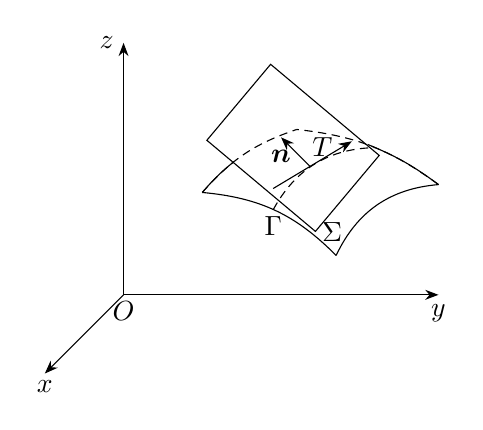
\begin{tikzpicture}[>=Stealth]
\draw[->](0,0)node[below=-1pt]{$O$}--(4,0)node[below]{$y$};
\draw[->](0,0)--(0,3.2)node[left]{$z$};
\draw[->](0,0)--(-1,-1)node[below=-1pt]{$x$};
\coordinate(a)at(1,1.3);\coordinate(b)at(2.7,0.5);
\coordinate(c)at(4,1.4);\coordinate(d)at(2.2,2.1);
\draw[bend left=20](a)to(b);
\draw[bend left=30](b)to(c);
\draw[densely dashed,bend left=15](a)to(d);
\draw[densely dashed,bend right=15](c)to(d);
\draw[bend left,densely dashed](1.9,1.08)node[below=-1pt](gamma){$\Gamma$}to(3.2,1.87);
\draw[->,xshift=-1mm,yshift=0.5mm](2,1.3)node(A){}--(3,1.9)node(B)[left,very near end]{$T$};
\draw[->](2.37,1.63)--(2,2)node[below=1pt]{$\bd n$};
\node[above]at(2.65,0.55){$\Sigma$};
\draw[rotate around={-40:(2.45,1.63)},scale=0.9,yshift=2mm](1.3,2.3)--(1.3,0.9)--(3.3,0.9)--(3.3,2.3)--cycle;
\draw[bend left=5](a)to(1.4,1.69);
\draw[bend right=7](c)to(3.1,1.91);
\end{tikzpicture}
 \newcounter{density}
  \setcounter{density}{20}
\begin{tikzpicture}
  \def\couleur{green!20!yellow}
  \path[coordinate] (0,0) coordinate(A)
              ++( 90:4cm) coordinate(B)
              ++(0:4cm) coordinate(C)
              ++(-90:4cm) coordinate(D);
  \draw (A) node[left] {A}
    (B) node[left] {B}
    (C) node[right] {Point C} --
    (D) node[right,midway,align=left] {边长$a$ \\ 面积和:$S=\frac{50}{9}a^2$ \\ 边长和:$C=\frac{20}{9}(10+\sqrt{82})a$}
    node[right] {点D};
  \draw[fill=\couleur!\thedensity] (A)--(B)--(C)--(D)--cycle;
  \foreach \x in {1,...,40}{%
      \pgfmathsetcounter{density}{\thedensity+25}
      \setcounter{density}{\thedensity}
      \path[coordinate] coordinate(X) at (A){};
      \path[coordinate] (A) -- (B) coordinate[pos=.1](A)
                          -- (C) coordinate[pos=.1](B)
                          -- (D) coordinate[pos=.1](C)
                          -- (X) coordinate[pos=.1](D);
      \draw[fill=\couleur!\thedensity] (A)--(B)--(C)--(D)--cycle;
  }
\end{tikzpicture}
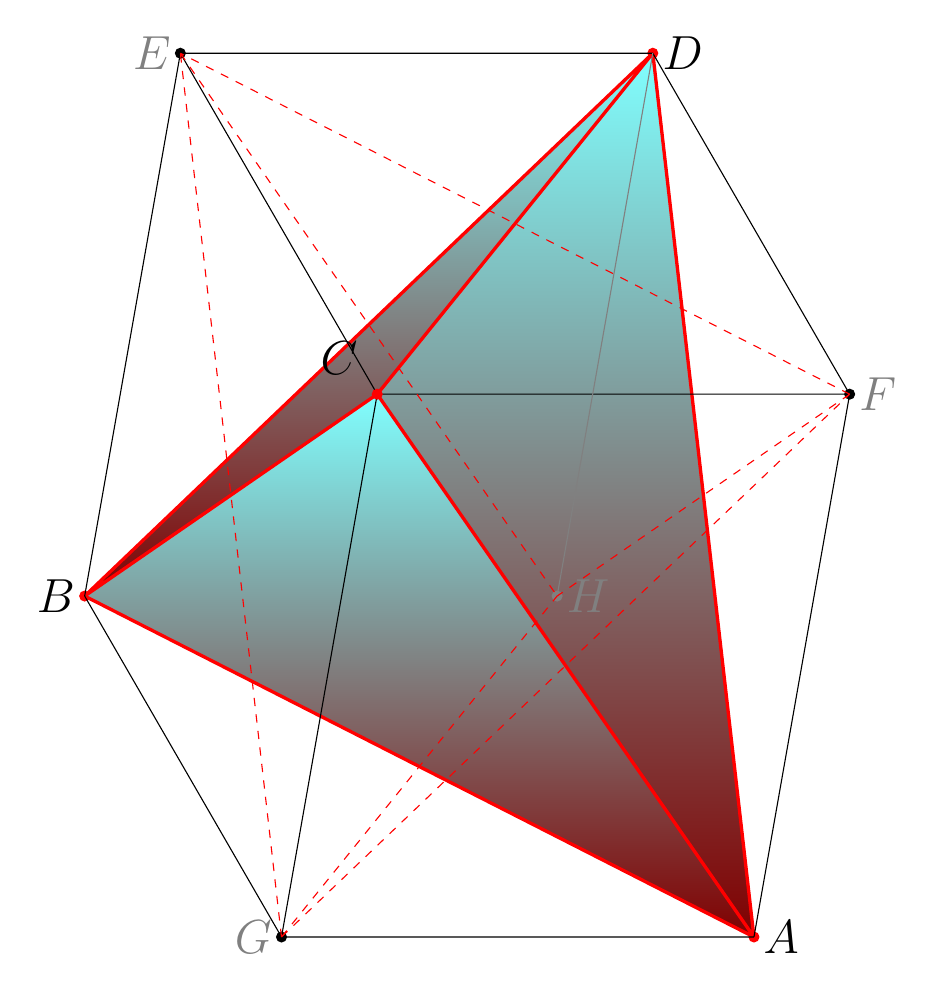
\begin{tikzpicture}[font=\LARGE]
\def \tta{ -10.00000000000000 } % Defines the first angle of perspective
\def \k{    -3.00000000000000 } % Factor for second angle of perspective
\def \l{     6.00000000000000 } % Defines the width  of the parallelepiped
\def \d{     5.00000000000000 } % Defines the depth  of the parallelepiped
\def \h{     7.00000000000000 } % Defines the heigth of the parallelepiped
\coordinate (A) at (0,0);
\coordinate (B) at ({-\h*sin(\tta)},{\h*cos(\tta)});
\coordinate (C) at ({-\h*sin(\tta)-\d*sin(\k*\tta)},
                    {\h*cos(\tta)+\d*cos(\k*\tta)});
\coordinate (D) at ({-\d*sin(\k*\tta)},{\d*cos(\k*\tta)});
\coordinate (Ap) at (\l,0);
\coordinate (Bp) at ({\l-\h*sin(\tta)},{\h*cos(\tta)});
\coordinate (Cp) at ({\l-\h*sin(\tta)-\d*sin(\k*\tta)},
                     {\h*cos(\tta)+\d*cos(\k*\tta)});
\coordinate (Dp) at ({\l-\d*sin(\k*\tta)},{\d*cos(\k*\tta)});
\fill[black]  (A) circle [radius=2pt];
\fill[red]    (B) circle [radius=2pt];
\fill[black]  (C) circle [radius=2pt];
\fill[red]    (D) circle [radius=2pt];
\fill[red]   (Ap) circle [radius=2pt];
\fill[black] (Bp) circle [radius=2pt];
\fill[red]   (Cp) circle [radius=2pt];
\fill[black] (Dp) circle [radius=2pt];
\filldraw[draw=red,bottom color=red!50!black, top color=cyan!50]
  (B) -- (Cp) -- (D);
\filldraw[draw=red,bottom color=red!50!black, top color=cyan!50]
  (B) -- (D)  -- (Ap);
\filldraw[draw=red,bottom color=red!50!black, top color=cyan!50]
  (B) -- (Cp) -- (Ap);
\draw[red,-,very thick] (Ap) --  (D)
                        (Ap) --  (B)
                        (Ap) -- (Cp)
                        (B)  --  (D)
                        (Cp) --  (D)
                        (B)  -- (Cp);
\draw [-,thin] (B)  --  (A)
               (Ap) -- (Bp)
               (B)  --  (C)
               (D)  --  (C)
               (A)  --  (D)
               (Ap) --  (A)
               (Cp) --  (C)
               (Bp) --  (B)
               (Bp) -- (Cp);
\draw [gray,-,thin] (Dp) -- (Cp);
                    (Dp) --  (D);
                    (Ap) -- (Dp);
\draw (Ap) node [right]           {$A$}
      (Bp) node [right, gray]     {$F$}
      (Cp) node [right]           {$D$}
      (C)  node [left,gray]       {$E$}
      (D)  node [left]            {$B$}
      (A)  node [left,gray]       {$G$}
      (B)  node [above left=+5pt] {$C$}
      (Dp) node [right,gray]      {$H$};
\fill[red]   (B) circle [radius=2pt];
\fill[gray] (Dp) circle [radius=2pt];
\draw[red,-,dashed, thin] (A)  -- (Dp)
                          (A)  -- (Bp)
                          (A)  --  (C)
                          (Bp) -- (Dp)
                          (C)  -- (Dp)
                          (Bp) --  (C);
\end{tikzpicture}
\setcounter{density}{20}
\begin{tikzpicture}
    \def\couleur{blue!10!green}
    \path[coordinate] (0,0)  coordinate(A)
                ++( 120:6cm) coordinate(B)
                ++(60:6cm) coordinate(C)
                ++(0:6cm) coordinate(D)
                ++(-60:6cm) coordinate(E)
                ++(240:6cm) coordinate(F)
                ;
    \draw[fill=\couleur!\thedensity] (A) -- (B) -- (C) --(D) -- (E) -- (F)-- cycle;
    \foreach \x in {1,...,60}{%
        \pgfmathsetcounter{density}{\thedensity+10}
        \setcounter{density}{\thedensity}
        \path[coordinate] coordinate(X) at (A){};
        \path[coordinate] (A) -- (B) coordinate[pos=.10](A)
                            -- (C) coordinate[pos=.10](B)
                            -- (D) coordinate[pos=.10](C)
                            -- (E) coordinate[pos=.10](D)
                             -- (F) coordinate[pos=.10](E)
                            -- (X) coordinate[pos=.10](F);
        \draw[fill=\couleur!\thedensity] (A)--(B)--(C)-- (D) --(E) -- (F) -- cycle;
    }
\end{tikzpicture}
\tikz\draw[ball color=red,shading=ball] (4,1) ..controls +(120:2cm)
        and +(90:2cm) .. (0,0) .. controls  +(-90:2cm) and +(90:3cm) ..
        (4,-8) .. controls +(90:3cm) and +(-90:2cm) ..(8,0)  .. controls
        +(90:2cm) and  +(60:2cm) .. (4,1);

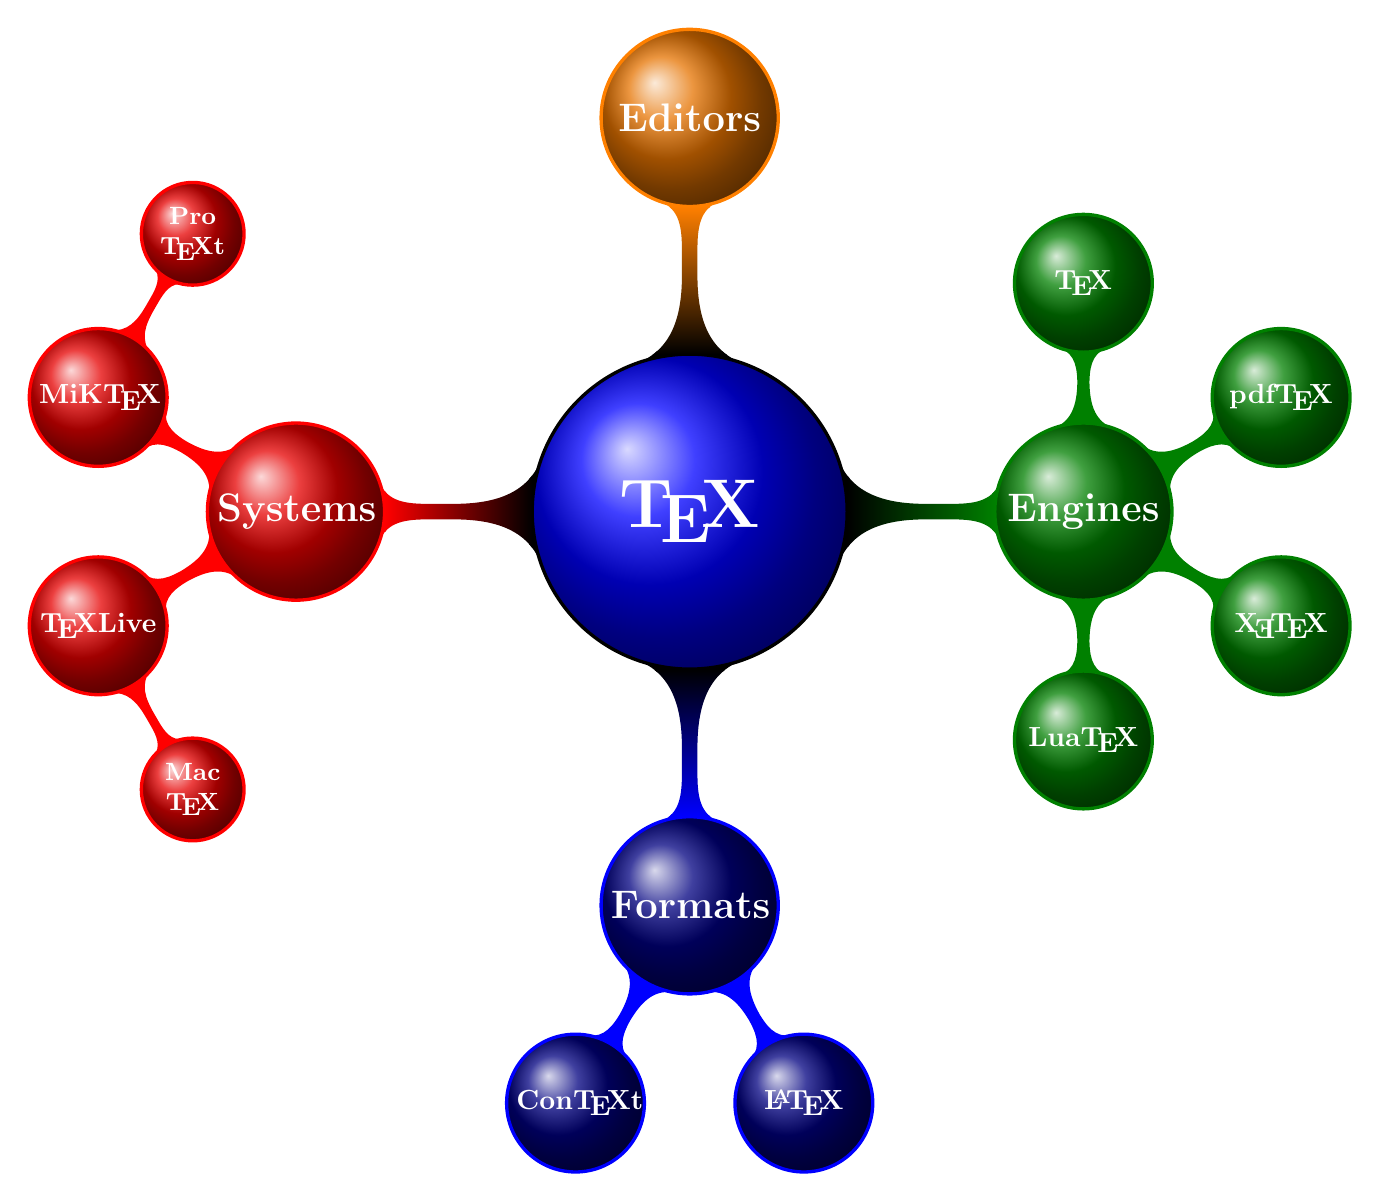
\begin{tikzpicture}
  \path [
    mindmap,
    text = white,
    level 1 concept/.append style =
      {font=\Large\bfseries, sibling angle=90},
    level 2 concept/.append style =
      {font=\normalsize\bfseries},
    level 3 concept/.append style =
      {font=\small\bfseries},
    tex/.style     = {concept, ball color=blue,
      font=\Huge\bfseries},
    engines/.style = {concept, ball color=green!50!black},
    formats/.style = {concept, ball color=blue!50!black},
    systems/.style = {concept, ball color=red!90!black},
    editors/.style = {concept, ball color=orange!90!black}
  ]
  node [tex] {\TeX} [clockwise from=0]
    child[concept color=green!50!black, nodes={engines}] {
      node {Engines} [clockwise from=90]
        child { node {\TeX} }
        child { node {pdf\TeX} }
        child { node {\XeTeX} }
        child { node {Lua\TeX} }}
    child [concept color=blue, nodes={formats}] {
      node {Formats} [clockwise from=300]
        child { node {\LaTeX} }
        child { node {Con\TeX t} }}
    child [concept color=red, nodes={systems}] {
      node {Systems} [clockwise from=210]
        child { node {\TeX Live} [clockwise from=300]
          child { node {Mac \TeX} }}
        child { node {MiK\TeX} [clockwise from=60]
          child { node {Pro \TeX t} }}}
    child [concept color=orange, nodes={editors}] {
      node {Editors} };
\end{tikzpicture}
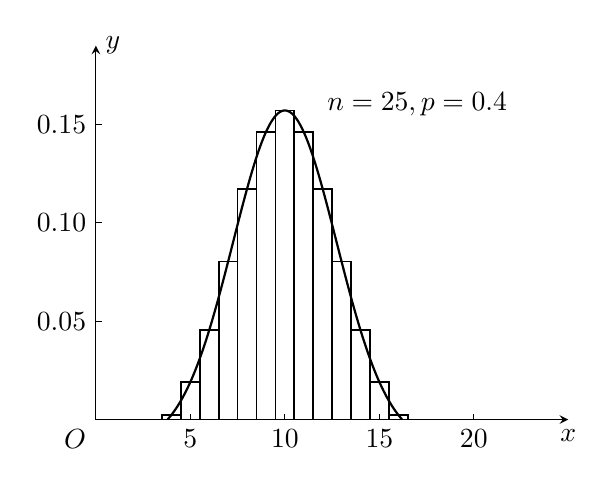
\begin{tikzpicture}[>=stealth,xscale=0.24,yscale=25]
\draw[->](0,0)node[below left]{$O$}--(25,0)node[below]{$x$};
\draw[->](0,0)--(0,0.19)node[right]{$y$};
\foreach \x in {5,10,15,20}\draw(\x,0)node[below]{$\x$}--(\x,0.003);
\foreach \x in {0.05,0.10,0.15}\draw(0,\x)node[left]{$\x$}--(0.3,\x);
\draw[samples=150,domain=3.8:16.2,thick]plot(\x,{0.17*e^(-(\x-10)^2/15)-0.013});
\foreach \x in {4,5,...,16}
\draw[semithick](\x-0.5,0)--(\x-0.5,{0.17*e^(-(\x-10)^2/15)-0.013})--
(\x+0.5,{0.17*e^(-(\x-10)^2/15)-0.013})--(\x+0.5,0)--cycle;
\node at(17,0.16){$n=25,p=0.4$};
\end{tikzpicture}

\definecolor{tou}{RGB}{94,125,89}
\definecolor{author}{RGB}{225,244,225}
\definecolor{title}{RGB}{255,253,127}
\definecolor{left}{RGB}{148,176,107}
\definecolor{body}{RGB}{144,192,108}
\definecolor{body1}{RGB}{90,182,90}
\definecolor{topbot}{RGB}{60,92,76}
\newcommand{\yp}[1]{{\CJKfontspec{印品赤壁赋体}#1}}
\newcommand{\fz}[1]{{\CJKfontspec{方正黑体简体}#1}}
\newcommand{\ii}{\,\!\mathrm i\,\!}
\begin{tikzpicture}
\node[minimum width=17.7cm,minimum height=25cm,inner sep=0pt,outer sep=0pt,](box){};
\fill[body,top color=body1,bottom color=body](box.north west)--(box.north east)--(box.south east)--(box.south west)--cycle;
\draw[help lines,step=0.8cm,opacity=0.4](-8.85,-12.5)grid(8.85,12.5);
\node[align=center,text=author] at (box.center)
{\zihao{-2}\fz{向禹} \tikz{\draw(0.25,0.25)circle(0.25);\draw(0.25,0.25)circle(0.2);} \fz{译}
};
\fill[tou](-8.85,6.5)[bend left=25]to(8.85,10.8)--(box.north east)--(box.north west)--cycle;
\fill[left color=left,right color=tou](-8.85,6.5)[bend left=24]to(8.85,10.6)
--(8.85,9.6)[bend right=23]to(-8.85,6.5);
\node[text=title,align=center,scale=3]at(0,4){\fz{1994-2018年国际大学生}\\[-0.2cm]\fz{数学竞赛}};
\node[text=orange!20,align=center,scale=1.5]at(0,2){\fz{International Mathematics Competition}\\[-0.2cm]\fz{for University Students (1994-2018)}};
\node[opacity=0.5,draw,rounded corners] at(-2,7.8){$\int_a^bf(x)\,\mathrm dx=F(b)-F(a)$};
\node[opacity=0.5] at(5.4,7.8){\tikz{\draw[-stealth](-0.3,0)--(0,0)node[below left]{$O$}--(3.6,0)node[below=2pt]{$x$};
\draw[-stealth](0,-0.42)--(0,2)node[left]{$y$};
\draw(0,1.3)node[left]{$A$}..controls(1.4,0.6)and(2.2,2.4)..(2.8,1.7)node[right]{$B$}
--(2.8,0)node[below]{$C$};\node at(0.65,1.4){$f(x)$};}};
\node[opacity=0.6] at(-3.5,-3.5)
{
\scalebox{0.5}{\begin{tikzpicture}
  \path [
    mindmap,
    text = white,
    level 1 concept/.append style =
      {font=\Large\bfseries, sibling angle=90},
    level 2 concept/.append style =
      {font=\normalsize\bfseries},
    level 3 concept/.append style =
      {font=\small\bfseries},
    tex/.style     = {concept, ball color=white,
      font=\Huge\bfseries},
    分析/.style = {concept, ball color=purple!90!black},
    formats/.style = {concept, ball color=blue!50!black},
    systems/.style = {concept, ball color=red!90!black},
    editors/.style = {concept, ball color=orange!90!black}
  ]
  node [tex,text=blue!80] {\scalebox{1.4}{IMC}} [clockwise from=0]
    child[concept color=green!50!black, nodes={分析}] {
      node {分析} [clockwise from=90]
        child { node {数学分析} }
        child { node {实分析} }
        child { node {复分析} }
        child { node {泛函分析} }
        }
    child [concept color=red, nodes={systems}] {
      node {图论组合}}
    child [concept color=blue, nodes={formats}] {
      node {代数} [clockwise from=240]
        child { node {线性代数} }
        child { node {抽象代数} }
         child { node {初等数论} }}
    child [concept color=orange, nodes={editors}] {
      node {概率论} };
\end{tikzpicture}}
};
\node[opacity=0.4]at(5.5,-2){
\begin{tikzpicture}[scale=10]
\begin{scope}
\clip (0,0) arc (-90:0:1/8) arc (90:180:1/8);
\fill[pattern=horizontal lines]
(0,0) arc (-90:0:1/8) --(1/16,1/16) arc (90:0:1/16);
\fill[pattern=vertical lines]
(0,0) arc (180:90:1/8) --(1/16,1/16) arc (0:90:1/16);
\end{scope}\node[below left](0,0){$O$};
\draw [-stealth](-1/8,0)--(0.34,0);\draw [-stealth](0,-1/8)--(0,0.34);
\node[below]at(0.34,0){$x$};\node[left]at(0,0.34){$y$};
\draw (0,0) arc (-90:90:1/8) (0,0) arc (-90:90:1/16)
(0,0) arc (180:0:1/8) (0,0) arc (180:0:1/16) (0,0)--(1/8,1/8);
\fill[fill=body](0.085,0.085)node[inner sep=0pt]{$D$}circle(0.01);
\draw(0,1/8)circle(1/8);\draw(0,1/16)circle(1/16);
\draw(1/8,0)circle(1/8);\draw(1/16,0)circle(1/16);
\node[above left]at(0,1/4){$\tfrac12$};\node[above left]at(0,1/8){$\tfrac14$};
\end{tikzpicture}
};
\node[opacity=0.3] at(3,-6.5){$\left( \sum_{n=1}^{\infty}{a_{n}^{2}} \right) \left( \sum_{n=1}^{\infty}{b_{n}^{2}} \right) \geqslant \left( \sum_{n=1}^{\infty}{a_nb_n} \right) ^2$};
\node[opacity=0.3] at(0,-8){$f(z)=\frac1{2\pi\ii}\oint_C\frac{f(\xi)}{\xi-z}\,\mathrm d\xi$};
\fill[tou](-8.85,-10.5)--(-8.85,-12.5)--(8.85,-12.5)--(8.85,-10.5)--cycle;
\node[anchor=north,align=left,text=author]at(0,-10.7){
\begin{tikzpicture}[color=author]
\draw[very thick,rounded corners](0,0)--(0,1.3)--(1.3,1.3)--(1.3,0)--cycle;
\fill(0.65,1.08)circle(0.12);
\fill(0.15,0.93)--(0.65,0.8)--(1.15,0.93)--(1.15,0.98)--(0.65,0.85)--(0.15,0.98)--cycle;
\foreach \x in{-0.12cm,-0.16cm,-0.2cm}
\fill[yshift=\x](0.15,0.93)--(0.65,0.8)--(1.15,0.93)--(1.15,0.98)--(0.65,0.85)
--(0.15,0.98)--cycle;
\foreach \x in{-0.32cm,-0.36cm,-0.4cm,-0.44cm,-0.48cm,-0.52cm,-0.56cm,-0.6cm,-0.64cm}
\fill[yshift=\x](0.15,0.93)--(0.65,0.8)--(1.15,0.93)--(1.15,0.98)--(0.65,0.85)
--(0.15,0.98)--cycle;
\end{tikzpicture}
\parbox{4cm}{\vspace{-1.2cm}
\scalebox{1.7}{\yp{无名出版社}}\\[-2mm]
\scalebox{0.5}[1]{PUBLISHING HOUSE OF NONAME}\\[-2mm]
\href{yuxtech.github.io}{yuxtech.github.io}
}};
\end{tikzpicture}

\end{document} 